\chapter{Simulations}\label{c:simulations}

In this chapter we present three different simulations. Two of which have an accompaning experimental data for micro tensile loading in the $[1\, 0\, 0]$ and $[1\, 1\, 0]$ directions of a single crystal Zn micropilar provided by Alan Xu from ANSTO Sidney. The third is is a proof of concept for a techinque developed by Jicheng Gong to cyclicly load a cantilever in opposing directions. However, this technique was developed on Ti microcantilevers and the HCP mobility law requires some adaptation before it is ready for general use. Instead we use the BCC law developed in-house by Bruce Bromage that as mentioned in the footnotes of \cref{ss:matrix}.

\section{Zinc tensile cantilever}\label{s:zincTensile}
\subsection{Introduction}
\subsection{Methodology}

\Cref{f:tensileSetup}
\begin{figure}
    \centering
    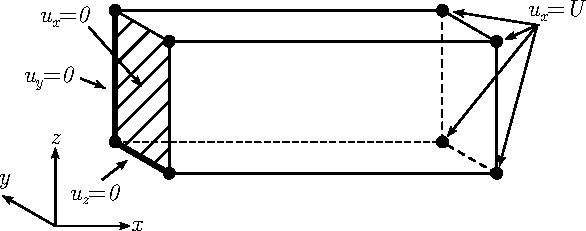
\includegraphics[width=0.8\linewidth]{tensileSetup.pdf}
    \caption[Displacement boundary conditions for dislocation plasticity modelling of single crystal micro-tensile tests.]{Displacement boundary conditions for dislocation plasticity modelling of single crystal micro-tensile tests.}
    \label{f:tensileSetup}
\end{figure}

\subsection{Results and discussion}
\subsection{Conclusions}

\section{Tungsten cyclic loading and unloading cantilever}\label{s:tungstenCyclic}
\subsection{Introduction}
\subsection{Methodology}
\subsection{Results and discussion}
\subsection{Conclusions}